% !TeX program = pdfLaTeX
\documentclass[12pt]{article}
\usepackage{amsmath}
\usepackage{graphicx,psfrag,epsf}
\usepackage{enumerate}
\usepackage{natbib}
\usepackage{textcomp}
\usepackage[hyphens]{url} % not crucial - just used below for the URL
\usepackage{hyperref}
\providecommand{\tightlist}{%
  \setlength{\itemsep}{0pt}\setlength{\parskip}{0pt}}

%\pdfminorversion=4
% NOTE: To produce blinded version, replace "0" with "1" below.
\newcommand{\blind}{0}

% DON'T change margins - should be 1 inch all around.
\addtolength{\oddsidemargin}{-.5in}%
\addtolength{\evensidemargin}{-.5in}%
\addtolength{\textwidth}{1in}%
\addtolength{\textheight}{1.3in}%
\addtolength{\topmargin}{-.8in}%

%% load any required packages here





\begin{document}


\def\spacingset#1{\renewcommand{\baselinestretch}%
{#1}\small\normalsize} \spacingset{1}


%%%%%%%%%%%%%%%%%%%%%%%%%%%%%%%%%%%%%%%%%%%%%%%%%%%%%%%%%%%%%%%%%%%%%%%%%%%%%%

\if0\blind
{
  \title{\bf Bringing Visual Inference to the Classroom}

  \author{
        Adam Loy \\
    Department of Mathematics and Statistics, Carleton College\\
      }
  \maketitle
} \fi

\if1\blind
{
  \bigskip
  \bigskip
  \bigskip
  \begin{center}
    {\LARGE\bf Bringing Visual Inference to the Classroom}
  \end{center}
  \medskip
} \fi

\bigskip
\begin{abstract}
In the classroom, we traditionally visualize inferential concepts using
static graphics or interactive apps. For example, there is a long
history of using apps to visualize sampling distributions. The lineup
protocol for visual inference is a recent development in statistical
graphics that has created an opportunity to hone student understanding.
Lineups are created by embedding plots of observed data into a field of
null (noise) plots. This arrangement facilitates comparison and helps
build student intuition about the difference between signal and noise.
Lineups can be used to visualize randomization/permutation tests,
diagnose models, and even conduct valid inference when distributional
assumptions break down. This paper provides an overview of how the
lineup protocol for visual inference can be used to build understanding
of key statistical topics throughout the statistics curricula.
\end{abstract}

\noindent%
{\it Keywords:} Statistical graphics, Simulation-based
inference, Visualizing uncertainty, Lineup protocol, Introductory
statistics, Model diagnostics
\vfill

\newpage
\spacingset{1.45} % DON'T change the spacing!

\hypertarget{introduction}{%
\section{Introduction}\label{introduction}}

Recent years have seen a great deal of innovation in how we teach
statistics as we strive to overcome what \citet{Cobb-2007uo} termed
``the tyranny of the computable.'' Most notably, simulation-based
pedagogies for the first course have been proposed and tested
\citep{Cobb-2007uo, Tintle-2011vo, Tintle-2012td, Maurer-2014te, Tintle2014-vt, Hildreth2018}.
These simulation-based pedagogies have also been used in mathematical
statistics \citep{chihara2011, Cobb2011-vz} and \citet{Tintle2015-yv}
argue that they should be used throughout the entire curriculum.

In addition to changes in how we introduce inference, there have also
been changes to the computational toolkit we use throughout the
statistics curriculum. At the introductory level, numerous toolkits are
commonplace depending on the objectives and audience of the course. Web
apps are commonly used when students may not have access to their own
computers, or simply to lower the technical barriers to entry. Examples
include StatKey \citep{Lock2017}, the \emph{Introduction to Statistical
Investigations} applets \citep{tintle2015}, and the Shiny apps from
\citet{agresti2017}. These apps allow students to explore course
concepts without getting into the computational weeds. For courses
exploring both the concepts and implementation in a realistic
data-analytic workflow, R \citep{r} is a common open-source choice and
multiple R packages have been developed to lower the barriers to entry
for students, notably mosaic \citep{Pruim2017-uc}, ggformula
\citep{ggformula}, and infer \citep{infer}.

The above developments enabled the statistics education community to
address key recommendations made in the GAISE report \citep{gaise2016}.
The simulation-based curriculum has focused attention on teaching
statistical thinking and fostering conceptual understanding before
delving into the mathematical details. An improved computational toolkit
has enabled students to use technology to explore concepts, such as a
sampling and permutation distributions, and to analyze data.

While the use of the simulation-based curriculum has helped students
focus on the underlying ideas of statistical inference, little has
changed about the way we help students \emph{visualize} inference.
Specifically, we still have students grapple with null/reference
distributions in hypothesis testing and sampling distributions for
estimation while they are trying to hone their intuition. These
distributions are very abstract ideas and while the web apps we use to
demonstrate their construction can help make sense of a single ``dot''
on the distribution, students commonly lose the forest for the trees.
\citet{wild2017} proposed the use of scaffolded animations to help
students hone their intuition about sampling/randomization variation and
to discover the utility of the bootstrap and permutation distributions.
While the animations discussed by \citet{wild2017} to visualize
randomization variation appear to be quite useful in communicating this
complex idea to students, a ``formal'' distribution is not necessary to
introduce the core ideas behind hypothesis testing. As an alternative,
we propose use of the lineup protocol \citep{Buja-2009bd} to visually
introduce the logic behind hypothesis tests and to help students
differentiate signal from noise as they meet new plots. Lineups are
created by generating a number of decoy plots and randomly situating the
data plot into this grid of plots. Using this lineup of plots, students
can be asked to apply ``Sesame Street logic'' (i.e., ``which one of
these is not like the others''), which can then be linked to fundamental
statistical ideas.

In this article, we discuss how to use the lineup protocol from visual
inference to help students differentiate between different forms of
signal and noise and to better understand the meaning of statistical
significance, or ``statistically discernible differences'' following the
suggestion of \citet{Witmer2019-qg}. Section \ref{sec:vizinf} presents
an overview of the lineup protocol. Section \ref{sec:intro} presents
examples of how the lineup protocol can be used in the first course, and
Section \ref{sec:othercourses} presents additional examples of its use
throughout the curriculum. In Section \ref{sec:implement} we discuss
implementation issues and informal student reactions. We conclude with a
brief summary in Section \ref{sec:conclusion}.

\hypertarget{visual-inference}{%
\section{Visual inference}\label{visual-inference}}

\label{sec:vizinf}

Most introductory statistics books teach that classical hypothesis tests
can be broken down into the following steps:

\begin{enumerate}
\def\labelenumi{\arabic{enumi}.}
\tightlist
\item
  Formulate competing claims, the null and alternative hypotheses.
\item
  Calculate a test statistic from the observed data.
\item
  Compare the test statistic to the reference (null) distribution.
\item
  Quantify the strength of evidence against the null by calculating a
  p-value.
\item
  State a conclusion in the context of the problem.
\end{enumerate}

\noindent This is still true for the first course after adapting it
based on the new GAISE guidelines, regardless of whether a
simulation-based approach is used
\citep{Lock2017, tintle2015, introstats}. In visual inference, the
\emph{lineup protocol} provides a direct analog for each step of a
hypothesis test \citep{Buja-2009bd}.

\begin{enumerate}
\def\labelenumi{\arabic{enumi}.}
\item
  \textbf{Competing claims}: As in a traditional hypothesis test, a
  visual test begins by clearly stating the competing claims about the
  model/population parameters.
\item
  \textbf{Test statistic}: A plot displaying the raw data or fitted
  model (called the \emph{observed plot}) serves as the test statistic.
  This plot must be chosen to highlight features of the data/model that
  are relevant to the hypotheses. For example, a scatterplot is a
  natural choice to examine whether or not two quantitative variables
  are correlated.
\item
  \textbf{Reference (null) distribution}: \emph{Null plots} are
  generated consistently with the null hypothesis and the set of all
  null plots constitutes the \emph{reference} (or \emph{null})
  \emph{distribution}. To facilitate comparison of the observed plot to
  the null plots, the observed plot is randomly situated in the field of
  null plots, just as a suspect is randomly situated among decoys in a
  police lineup. This arrangement of plots is called a \emph{lineup}.

  \emph{Technical note:} When introducing the lineup to our students we
  tell them that the null plots were generated in a manner such that the
  null hypothesis is true, glossing over additional details/conditions
  to focus student attention focus on the main point of the hypotheses.
  For example, using permutation resampling to investigate a difference
  in means requires not only that the means of the two distributions are
  equal, but that the two groups have the same distribution, so the
  spread and shapes of the distributions must also be the same. When you
  discuss the details behind the permutation test you can return to the
  lineups to clarify this point, but students don't need that level of
  detail when initially building their intuition.
\item
  \textbf{Assessing evidence}: If the null hypothesis is true, then we
  expect the observed plot to be indiscernible from the null plots. The
  more discernible the observed plot is from the lineup, the more
  evidence this provides against the null hypothesis. If one wishes to
  calculate a visual p-value, then lineups need to be presented to a
  number of independent observers for evaluation. While this is
  possible, it is not a productive discussion in introductory courses
  that don't explore probability theory.
\item
  \textbf{Stating a conclusion}: A visual test, just like a traditional
  hypothesis test, ends by interpreting the evidence and stating a
  conclusion.
\end{enumerate}

\hypertarget{example-comparing-groups}{%
\subsection{Example: Comparing groups}\label{example-comparing-groups}}

As a first example of visual inference via the lineup protocol, consider
the creative writing experiment discussed by \citet{ramsey2013}. The
experiment was designed to explore whether motivation type (intrinsic or
extrinsic) impacted creativity scores. To evaluate this, creative
writers were randomly assigned to a questionnaire where they ranked
reasons they write: one questionnaire listed intrinsic motivations and
the other listed extrinsic motivations. After completing the assigned
questionnaire, all subjects wrote a Haiku about laughter, which was
graded for creativity by a panel of poets. \citet{ramsey2013} discuss
how to conduct a permutation test for the difference in mean creativity
scores between the two treatment groups. Below, we illustrate the steps
of a visual test.

\begin{enumerate}
\def\labelenumi{\arabic{enumi}.}
\item
  A visual test begins identically to a traditional hypothesis test by
  clearly stating the competing claims about the model/population
  parameters. In a first course, this could be written as:
  \(H_0: \mu_{\rm intrinsic} - \mu_{\rm extrinsic} = 0\)
  vs.~\(H_0: \mu_{\rm intrinsic} - \mu_{\rm extrinsic} \ne 0\).
\item
  In a visual test, plots take the role of test statistics
  \citep{Buja-2009bd}. In this situation, we must choose a plot that can
  highlight the difference in average creativity scores between the
  intrinsic and extrinsic treatment groups. Figure \ref{fig:data_plot}
  displays boxplots of creative writing scores by treatment group where
  a dot is used to represent the sample mean for each group, though
  other graphics could be used. There is an apparent difference in the
  distribution of the scores---the average score for the intrinsic group
  appears to be larger---but could it be due to chance alone?

  \begin{figure}
  \centering
  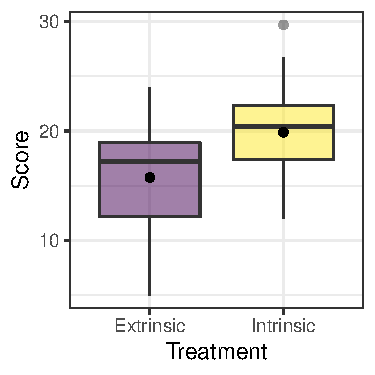
\includegraphics{figs/diff_means_plot.pdf}
  \caption{\label{fig:data_plot} Boxplots of the original creative
  writing scores by treatment group. The dot represents the mean of each
  group.}
  \end{figure}
\item
  To understand whether the observed (data) plot provides evidence of a
  statistically discernible difference, we must understand the behavior
  of our test statistic under the null hypothesis. To do this, we
  generate \emph{null plots} consistent with the null hypothesis and the
  set of all null plots constitutes the reference distribution. To
  facilitate comparison of the data plot to the null plots, the data
  plot is randomly situated in the field of null plots. This arrangement
  of plots is called a \emph{lineup}. Figure \ref{fig:lineup} shows one
  possible lineup for the creative writing experiment. The nineteen null
  plots were generated via permutation resampling, and the data plot was
  randomly assigned to panel \#10.

  \begin{figure}
  \centering
  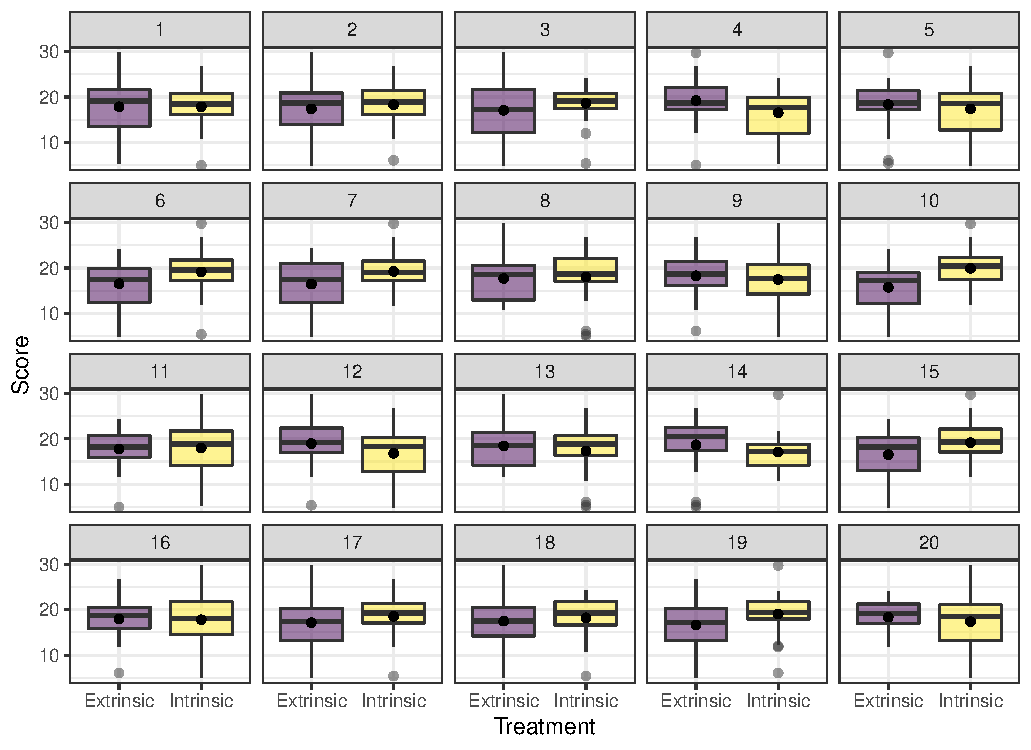
\includegraphics{figs/permute_lineup.pdf}
  \caption{\label{fig:lineup} A lineup consisting of 19 null plots
  generated via permutation resampling and the original data plot for
  the creative writing study. The data plot was randomly placed in panel
  \#10. Can you discern the difference?}
  \end{figure}
\item
  If the null hypothesis is true, then we expect the data plot to be
  indiscernible from the null plots. Thus, if one is able to identify
  the data plot in panel \#10 of Figure \ref{fig:lineup}, then this
  provides evidence against the null hypothesis. We will not discuss the
  process of calculating a visual \(p\)-value, as the pedagogical value
  of the lineup protocol is in visualizing signal and noise.
\item
  Depending on your selection, you would either write a conclusion
  communicating that you found evidence of a discernible difference (or
  made a lucky guess), or did not find evidence of a discernible
  difference. Either way, this conclusion should be framed in context.

  \emph{Note:} With only one observer this binary result (identifying
  the data or not) can appear to reinforce the type of bright-line
  thinking that the statistics community is trying to avoid
  \citep{Wasserstein2016-al}. While this is a risk, it is mitigated by
  class discussion, as you will see below.
\end{enumerate}

\hypertarget{using-visual-inference-in-introductory-statistics}{%
\section{Using visual inference in introductory
statistics}\label{using-visual-inference-in-introductory-statistics}}

\label{sec:intro}

In this section, we discuss how to use the lineup protocol in the
introductory setting to introduce students to the logic of hypothesis
testing and to help students interpret new statistical graphics. The
goal is to provide examples of how this can be done, not to provide an
exhaustive list of possibilities.

\hypertarget{introducing-simulation-based-inference}{%
\subsection{Introducing (simulation-based)
inference}\label{introducing-simulation-based-inference}}

The strong parallels between visual inference and classical hypothesis
testing make it a natural way to introduce the idea of statistically
discernible differences (i.e., statistical significance) without getting
bogged down in minutiae/controversy of p-values, or the technical issues
of describing a simulation procedure before students understand why that
is important. All students understand the question ``which one of these
plots is not like the others,'' and this common understanding generates
fruitful discussion about the underlying inferential thought process
without the need for a slew of definitions. Below is an outline of a
class activity discussing the creative writing experiment to introduce
the inferential thought process.

\hypertarget{outline-of-activity}{%
\subsubsection{Outline of activity}\label{outline-of-activity}}

This activity is designed to be completed in groups of three or four
students. We have found that this group size allows all students to
contribute to the discussion, and is also conducive to assigned roles,
such as facilitator, spokesperson, recorder, and encourager/questioner
\citep[see][]{Garfield1993-oy, Roseth2008-xx}.

\textbf{Competing claims.} To begin, we have students discuss what
competing claims are being investigated. We encourage them to write
these in words before linking them with the mathematical notation they
saw in the reading prior to class. The most common answer is: ``there is
no difference in the average creative writing scores for the two groups
vs.~there is a difference in the average creative writing scores for the
two groups.'' During the debrief, we make sure to link this to the
appropriate notation.

\textbf{EDA review.} Next, we have students discuss what plot types
would be most useful to investigate this claim. It's important to ask
students why they selected a specific plot type, as this reinforces
links to key ideas from exploratory data analysis.

\textbf{Lineup evaluation.} Most students recognize that side-by-side
boxplots, faceted histograms, or overlayed density plots are reasonable
choices to display the relevant aspects of the distribution of creative
writing scores for each group. We then provide a lineup of side-by-side
boxplots to evaluate (we do place a dot at the sample mean for each
group), such as the lineup shown in Figure \ref{fig:lineup}. At this
point, we do not give the details behind the creation of null plots, we
simply tell students that one plot is the observed data while the other
nineteen agree with the null hypothesis. We ask students to choose which
plot is the most different from the others and explain why they chose
that plot. Once each student has had time to make this assessment
(usually about one or two minutes), we ask the groups to discuss and
defend their choices.

\textbf{Lineup discussion.} After all of the groups have evaluated the
lineup and discussed their reasoning, we regroup for a class discussion.
During this discussion, we reveal which panel contains the observed data
(panel \#10 of Figure \ref{fig:lineup}), and display these data on a
slide so that we can point to particular features of the plot as
necessary. After revealing the observed data, we have students return to
their groups to discuss whether they chose the real data and whether
their choices support either of the competing claims. Once the class
regroups and thoughts are shared, we make sure that the class realizes
that an identification of the observed data provides evidence against
the null hypothesis (though we always hope students will be the ones
saying this).

\hypertarget{interpreting-unfamiliar-plots}{%
\subsection{Interpreting unfamiliar
plots}\label{interpreting-unfamiliar-plots}}

You can also utilize the lineup protocol to introduce new and unfamiliar
plot types. For example, we have found many introductory students
struggle to interpret residual plots. In this situation, the lineup
protocol helps students tune their understanding of what constitutes an
``interesting'' pattern (i.e., signal).

\hypertarget{residual-plots}{%
\subsubsection{Residual plots}\label{residual-plots}}

Interpreting residual plots is fraught with common errors and we have
found that, regardless of our valiant attempts to explain what ``random
noise'' or ``random deviations from a model'' might look like, there is
no substitute for first-hand experience. In this section, we outline a
class activity/discussion designed to help train students to interpret
residual plots. This activity takes place after a brief introduction to
residual plots is given in class (or video if in a flipped or hybrid
classroom). Again, we suggest that students complete such an activity in
small groups.

\textbf{Model fitting.} To begin, we have students fit a simple linear
regression model, interpret the coefficients, write down what a residual
is (in both words and using notation), and calculate a residual for a
specific observation.

\textbf{Introduce residual plots.} Next, we define (or review) what a
residual plot is and ask students what conditions for regression could
be checked using this type of plot. At this point we do not have
students render a residual plot so that they can be asked ``which of
these residual plots is not like the others'' when evaluating a lineup.
Alternative versions of this activity could have students create the
residual plot first and then use a lineup to evaluate it.

\textbf{Lineup evaluation.} Once students have considered how to use a
residual plot, we have them generate via a Shiny app (or present them
with) a lineup of residual plots, such as the plot shown in Figure
\ref{fig:lineupresid}. Here, the null plots have been generated using
the parametric bootstrap, but the residual or non-parametric bootstraps
are other viable choices. We avoid the details of how the null plots
were generated, but this depends on the goals for your class. Once the
lineup has been generated, we ask students to identify which plot is
most different from the others, describe what feature(s) led them to
their choice and to choose two other plots (i.e., plots they think are
decoys) and describe any patterns they see. We ask students to answer
these questions individually before discussing them in their groups.
Typically about three to five minutes of ``think time''are given prior
to group discussion.

\begin{figure}
\centering
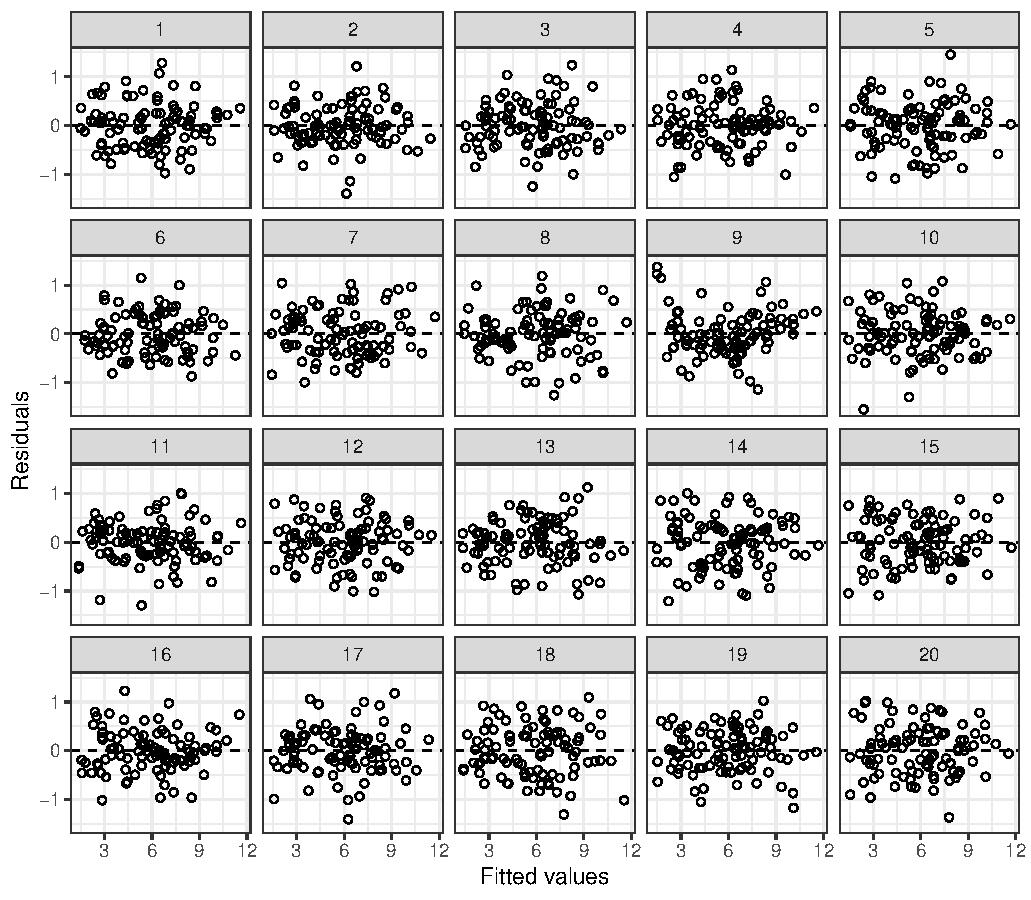
\includegraphics{figs/residual_lineup.pdf}
\caption{\label{fig:lineupresid} A lineup of residual plots. The null
plots are generated via a parametric bootstrap from the fitted model.
The observed data are shown in panel \#9. Can you discern the
difference?}
\end{figure}

\textbf{Debrief.} Once all of the groups have evaluated their lineups
and discussed their reasoning, it is important to regroup for a class
discussion. This allows you to reveal the observed residual plot and
revisit key points about residual plots and their interpretation. During
this process, we often have students return to their groups to discuss
the implications of their choice after they learn which panel was the
observed residual plot, after which we discuss the implications as a
class.

\textbf{Teaching tips}

\begin{itemize}
\item
  In Figure \ref{fig:lineupresid}, the observed residual plot in panel
  \#9 is systematically different from the null plots. While this is one
  example we use in class, we also recommend a parallel example where
  there is no discrepancy between the data and the model.
\item
  Depending on your course goals, follow-up discussions about the design
  of residual plots could be injected to the end of this activity. For
  example, you could provide students with a second version of the
  lineup where LOESS smoothers have been added to each panel and ask
  students what features of the residual plot the smoother highlights.
\item
  An alternative activity first has students use the
  \emph{Rorschach protocol} \citep{Buja-2009bd} to look through a series
  of null plots, describing what they see, and then has them look at a
  single residual plot.
\end{itemize}

\hypertarget{other-plot-types}{%
\subsubsection{Other plot types}\label{other-plot-types}}

Similar activities can be designed to introduce other statistical
graphics. Specifically, we have also found that lineups help students
learn to read normal quantile-quantile and mosaic plots (or stacked bar
charts).

\hypertarget{using-visual-inference-in-other-courses}{%
\section{Using visual inference in other
courses}\label{using-visual-inference-in-other-courses}}

\label{sec:othercourses}

The utility of visual inference is not limited to introductory courses.
Whenever a new model is encountered intuition about diagnostic plots
must be rebuilt, and the lineup protocol helps students build this
intuition. As an example, consider diagnostics for binary logistic
regression models, a common topic in a second course.

\hypertarget{diagnostics-for-binary-logistic-regression}{%
\subsection{Diagnostics for binary logistic
regression}\label{diagnostics-for-binary-logistic-regression}}

Interpreting residual plots from binary logistic regression is
difficult, as plots of the residuals against the fitted values or
predictors often look similar for adequate and inadequate models. The
lineup protocol provides a framework for this discussion. For example,
you can simulate data from a model where a quadratic effect is needed,
but fit the data to a model with only a linear effect and extract the
Pearson residuals. Then, you can simulate the null plots from the model
with only the linear effect and extract the Pearson residuals. Figure
\ref{fig:logisticissue} shows a lineup created in this way, and the
observed residual plot (panel \#8) does not appear to stand out from the
field of null plots. Having a discussion surrounding this lineup in
class will help pinpoint the difficulty of using ``conventional''
residual plots for model diagnosis.

\begin{figure}
\centering
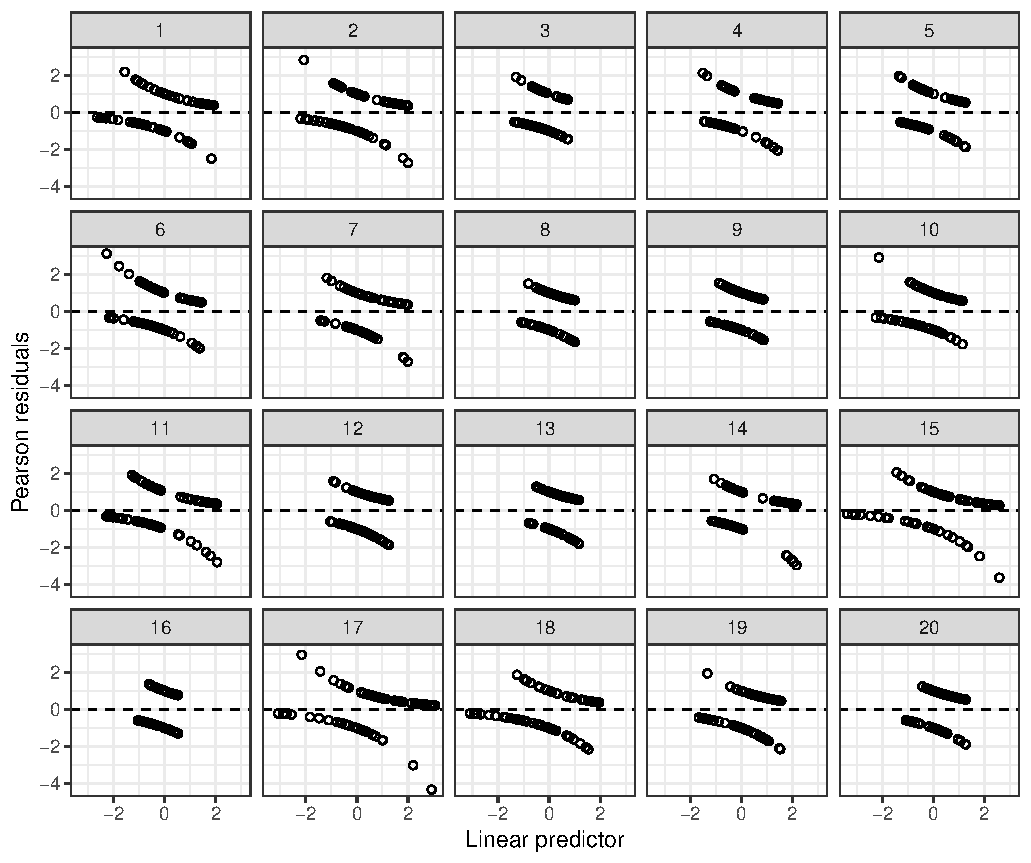
\includegraphics{figs/logistic_residuals_bad.pdf}
\caption{\label{fig:logisticissue} A lineup for a deficient logistic
regression model. The data plot are simulated from a model with a
quadratic effect, while the null plots are simulated from a model with
only a linear effect. Can you identify the deficient plot?}
\end{figure}

After establishing the pitfalls of ``conventional'' residual plots for
binary logistic regression, you can introduce alternative strategies
(i.e., new diagnostic plots) and again use the lineup protocol to
calibrate student intuition. Below are two such examples.

\hypertarget{binned-residual-plots}{%
\subsubsection{Binned residual plots}\label{binned-residual-plots}}

\citet{GelmanHill:2007} recommend using \emph{binned residual plots} to
explore possible violations of linearity for binary logistic regression.
A binned residual plot is created by calculating the average residual
value in bins that partition the \(x\)-axis. Figure \ref{fig:binned}
shows a binned residual plot from a simple binary logistic regression
model. The average deviance residual is plotted on the \(y\)-axis for
each of 54 bins on the \(x\)-axis. The number of bins is set to
\(\lfloor \sqrt{n} \rfloor\), but can be adjusted as with a histogram.
\citet{GelmanHill:2007} claim that these plots should behave much like
the familiar standardized residual plots from regression. If this claim
is true, then Figure \ref{fig:binned} is indicative of nonlinearity.
However, rather than simply citing \citet{GelmanHill:2007} to students,
a lineup empowers them to investigate the behavior of this new plot
type. A lineup for these residuals is given in Figure
\ref{fig:binnedlineup}. As suspected, the data plot (panel \#8) stands
out from the field of null plots, indicating a deficiency with the
model. This investigation via a lineup can be framed as a whole class
discussion or as a group activity, similar to the activities already
outlined.

\begin{figure}
\centering
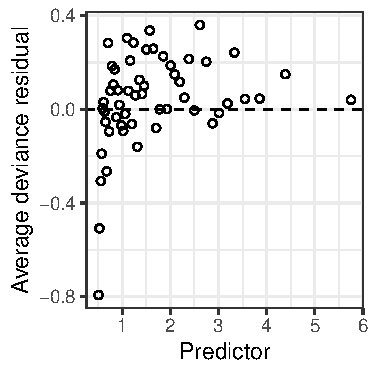
\includegraphics{figs/binned_resid_example.pdf}
\caption{\label{fig:binned} A binned residual plot from a simple binary
logistic regression model. The average deviance residual is plotted on
the \(y\)-axis for each of 54 bins on the \(x\)-axis.}
\end{figure}

\begin{figure}
\centering
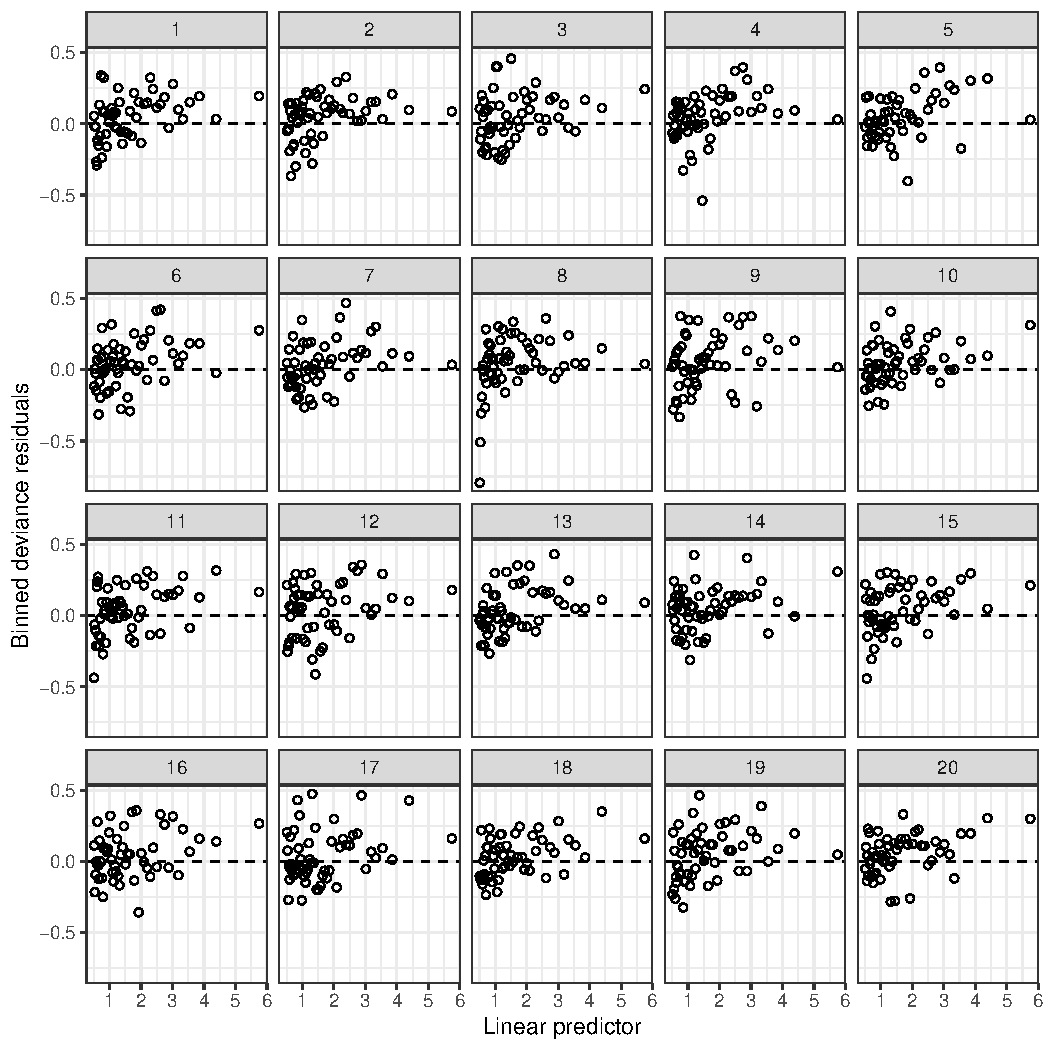
\includegraphics{figs/wells_binned_residuals.pdf}
\caption{\label{fig:binnedlineup} A lineup of binned residual plots from
a simple binary logistic regression model. The observed residuals are
shown in panel \#8 and clearly stand out from the field of null plots,
indicating a problem with linearity.}
\end{figure}

\hypertarget{empirical-logit-plots}{%
\subsubsection{Empirical logit plots}\label{empirical-logit-plots}}

A more-common alternative to the binned residual plot is the
\emph{empirical logit plot} \citep[c.f.,][]{stat2, ramsey2013}. An
empirical logit plot can be constructed for each explanatory variable by
calculating the adjusted proportion of ``successes'' within each
``group'' as \[
\widehat{p}_{\rm adj} = \frac{\text{number successes} + 0.5}{\text{number of cases} + 1},
\] and plotting
\(\log\left(\widehat{p}_{\rm adj} / (1- \widehat{p}_{\rm adj}) \right)\)
against the average value of a quantitative explanatory variable, or the
level of a categorical explanatory variable. For quantitative variables,
it is common to form groups by forming bins of roughly equal size.

While an empirical logit plot is quite straightforward to create, it can
be hard to interpret for smaller data sets where few groups are formed.
For example, \citet{stat2} use empirical logit plots to explore a binary
logistic regression model for medical school admission decisions based
on an applicant's average grade point average and render empirical logit
plots based on both 5 and 11 bins. Figure \ref{fig:emplogitexample}
shows recreations of these plots. Experimenting with the number of bins
reveals the difficulty students may encounter determining whether
linearity is reasonable: the plot can change substantially based on the
number of bins chosen. In our experience, students often see some
indication of non-linearity in the plot with 5 bins (Figure
\ref{fig:emplogitexample} (a)), whereas they think the plot with 11 bins
(Figure \ref{fig:emplogitexample} (b)) is reasonably linear.

\begin{figure}

{\centering 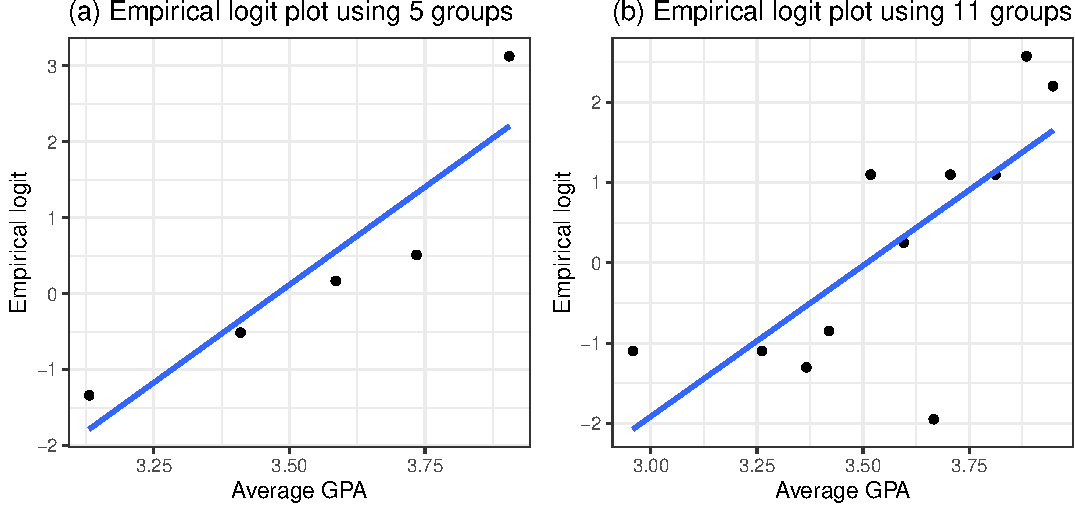
\includegraphics[width=0.85\linewidth]{vizinf-paper_files/figure-latex/unnamed-chunk-7-1} 

}

\caption{\label{fig:emplogitexample} Two empirical logit plots rendered for the same data set with $n=55$ observations. Panel (a) is rendered using 5 groups while panel (b) is rendered using 11 groups. The appearance of the plots changes substantially, often leading to confusion in intrepretation.}\label{fig:unnamed-chunk-7}
\end{figure}

\begin{figure}
\centering
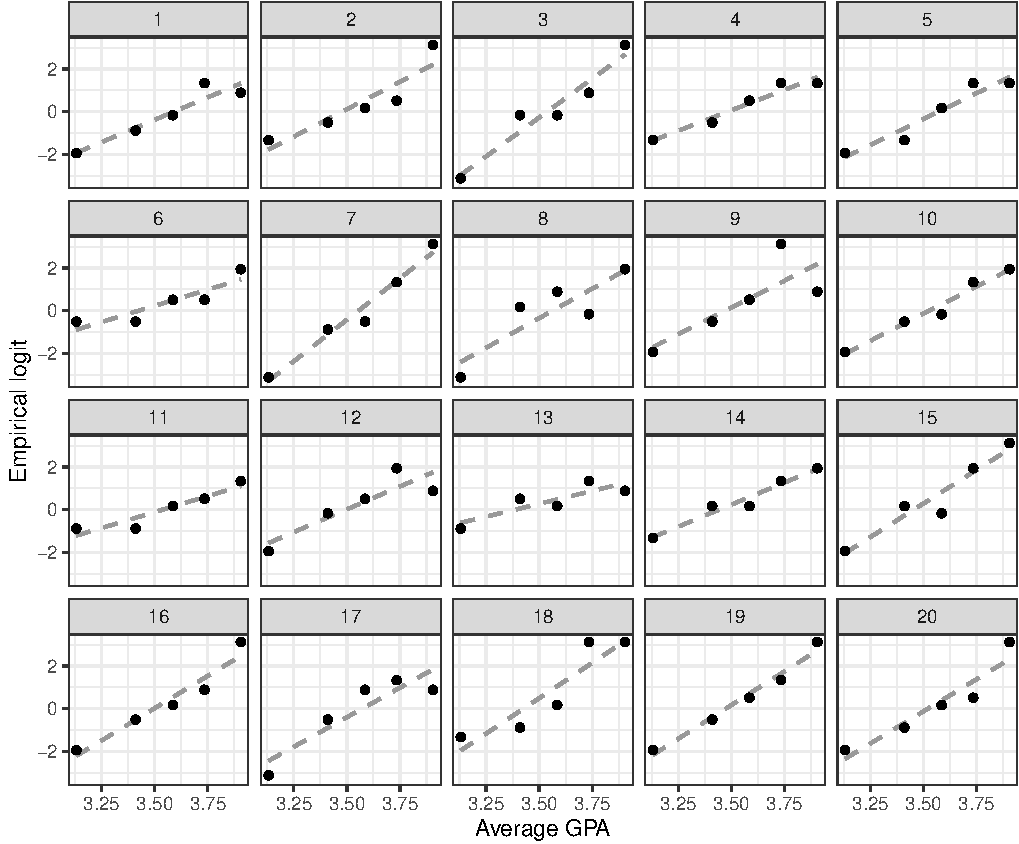
\includegraphics{vizinf-paper_files/figure-latex/unnamed-chunk-8-1.pdf}
\caption{\label{fig:emplogitlineup} A lineup of empirical logit plots
from a simple binary logistic regression model. The observed plot is
shown in panel \#2 and does not stand out from the field of null plots,
indicating no problem with linearity.}
\end{figure}

To help students interpret whether observed patterns on empirical logit
plots are problematic, we again appeal to the lineup protocol to force a
comparison between the observed plot and what is expected under the
model. Figure \ref{fig:emplogitlineup} displays a lineup of the
empirical logit plot created using 5 groups. The observed plot (panel
\#2) is difficult to pick out from the field of null plots, providing no
evidence against linearity.

\hypertarget{diagnosing-other-models}{%
\subsection{Diagnosing other models}\label{diagnosing-other-models}}

In this section, we focused on using the lineup protocol to help
diagnose logistic regression models, but the approach is generally
applicable. If you have a plot highlighting some feature(s) of the
fitted model, then after simulating data from a ``correct'' model (i.e.,
one without model deficiencies), you can create a lineup to interrogate
the model. For example, \cite{Loy2017-fo} discuss how visual inference
can be used to diagnose multilevel models.

\hypertarget{implementation-and-student-reception}{%
\section{Implementation and student
reception}\label{implementation-and-student-reception}}

\label{sec:implement}

\hypertarget{how-to-create-lineups}{%
\subsection{How to create lineups}\label{how-to-create-lineups}}

All of the lineups presented in this paper were rendered in R \citep{r}.
A tutorial outlining this process using the ggplot2 \citep{ggplot2} and
nullabor \citep{nullabor} R packages is provided in the supplementary
materials. These tools allow you to customize lineups for class use, but
we do not recommend having introductory students grapple with this code.
For introductory students, we recommend providing handouts or slides
with pre-rendered lineups during class activities. Alternatively, we
have created a suite of Shiny apps \citep{shiny} where students can
upload data sets and render lineups. The current suite includes apps to
generate lineups to explore associations between groups, normal Q-Q
plots, and residual plots for simple linear regression models. Links to
the Shiny apps can be found at
\url{https://aloy.github.io/classroom-vizinf/}.

\hypertarget{scaffolding-class-activities}{%
\subsection{Scaffolding class
activities}\label{scaffolding-class-activities}}

The lineup activities briefly outlined in Sections \ref{sec:intro} and
\ref{sec:othercourses} follow the same framework, which we briefly
expand on below. We have also included the full-length activities along
with instructor guides for the activities outlined in Section
\ref{sec:intro} in the supplementary material.

\emph{Introduce the main idea.} Before starting the activity, we
introduce students to the main idea via assigned reading or a mini
lecture. For example, to use a lineup to introduce mosaic plots,
students should first understand what a mosaic plot is. The first time
we utilize a lineup in class, we also provide a brief introduction of
what a lineup is, as discussed in Section \ref{sec:vizinf}. We typically
use in-class mini lectures to introduce the main idea, but recording
these mini lectures for pre-class viewing is an attractive option.

\emph{Setup questions.} The lineup activities contain a few questions
for students to discuss as a group before seeing a lineup. For example,
the activity in Section \ref{sec:intro} introducing the logic of testing
has students discuss the hypotheses, identify the response and
explanatory variables, and discuss what type of plot they would choose
to explore the data prior to examining a lineup. These questions help
make connections to previous topics, but also allow the group to work
together before discussing lineups. This seems to ``break the ice,'' and
has led to more engaged discussions.

\emph{Lineup evaluation and discussion.} Once a group has completed the
setup, students individually evaluate a lineup. We ask students to
choose which plot is the most different from the others and explain why
they chose that plot. Once each student has had time to make this
assessment (usually about one or two minutes) we ask the students to
discuss and defend their choices with their group. More time can be
given if you want students to write down their justification before
discussing their choice. We generally give between five and ten minutes
for this discussion, using cues from the class and our perception of the
lineup difficulty to determine whether to extend time past the initial
five minutes. To guide the group discussion it can be helpful to ask
specific questions, such as

\begin{itemize}
\tightlist
\item
  ``Which one of these plots is not like the others?''
\item
  ``What feature of the plot led you to this choice?''
\item
  ``What does your choice indicate about your initial claim?'' (if
  introducing hypothesis testing)
\item
  ``What does your choice indicate about the data?'' (if conducting EDA)
\item
  ``What does your choice indicate about the model conditions?'' (if
  interpreting diagnostic plots)
\end{itemize}

\noindent We have found having each group report back to the class leads
to far more productive conversations. In addition, assigning roles
eliminates the need to discuss who will report back to the class.

\emph{Reveal and discussion.} Next, have each group share their
selection and justification. This could be done by calling on each
group, or by tracking the choices of each group through post-it notes on
the board or a quick survey. If you choose the latter option, then
calling on a couple groups to justify their selections after tallying
the choices helps focus discussion. It is useful to have the lineup
projected during this discussion so that you can highlight specific
features mentioned. Once the groups have shared their selections, have
students return to their small groups to discuss the implications of
their selections.

\emph{Debriefing.} The final step of the activity is a class-wide
discussion. Each group (or a randomly chosen subset) can report back on
the implications of their choice. What these choices imply is the key
idea behind the activity, so it's important to spend time on this step.
We tend to give a mini lecture at the end recapping the main points of
both the activity and discussion to help students reflect on the
process. This part of the activity generally lasts about ten minutes,
but is variable depending on the talking points brought from the groups.

While we have found in-class activities exploring new plot types and the
inferential thought process to be useful, these could also be assigned
as homework problems or pre-class exercises. Regardless of the mode,
scaffolding the activity to guide students and foster
discussion/reflection is key. In the above examples, we illustrated the
approach that has worked well for our students, but each instructor
should adjust this to their own class, teaching style, and student
population. In addition, our discussion has not been exhaustive, so we
encourage instructors to identify additional places in their curriculum
where the lineup protocol can help their students build intuition.

\hypertarget{addressing-subjectivity}{%
\subsection{Addressing subjectivity}\label{addressing-subjectivity}}

Unless you only use lineups in situations where there are obvious
differences between groups or clear associations, you will encounter
situations where some students struggle to identify the data plot. While
this can be frustrating, we believe this is a productive struggle. We
have found the following strategies to be helpful in dealing with this
uncertainty:

\begin{itemize}
\item
  A first point of frustration is that each student has their own
  ability to perceive patterns/differences. Consequently, some students
  will need more time to evaluate lineups and some students will be
  unable to perceive smaller differences. A quick comment acknowledging
  the inherent differences in perceptual ability between people can
  diffuse some of this frustration. This acknowledgment can be followed
  by encouraging students to discuss the reasons plots were chosen and
  to come to consensus as a group. The discussions surrounding lineups
  help students see that they are not alone in their frustration, and
  discussing their thought processes with their peers helps them remain
  engaged rather than staring blankly at a plot.
\item
  During the debriefing session, have each group share their chosen plot
  and use differences of opinion as discussion opportunities. For
  example, one group may have focused on outliers while another focused
  on central tendency. That's an interesting difference that can lead to
  discussions of which plot to choose if you want to focus attention on
  specific features of a distribution. This discussion will also
  highlight that uncertainty still exists even if one person or group is
  able to discern the data plot.
\item
  When introducing the logic of testing, it is also valuable to design a
  lineup where everyone will struggle. This will help students visualize
  the situation where there is no association and can lead to fruitful
  discussions if a group chooses the data plot by chance alone. These
  lineups can later be talking points surrounding statistical errors.
\end{itemize}

A side benefit of students struggling with the uncertainty, and
sometimes difficulty, of identifying the data plot is that they are
primed for discussions that discourage bright-line thinking. If you have
already discussed the differences in individual perceptive ability, then
it is natural to challenge the idea of some ``universal cutoff'' for
strength of evidence.

\hypertarget{student-reception}{%
\subsection{Student reception}\label{student-reception}}

We have not formally tested the utility of lineups in the classroom, but
we can offer informal observations on how students responded to the
class activities. These observations are taken from two courses: an
introductory course and a second course in statistics. The introductory
course is taught out of \emph{Statistics: Unlocking the Power of Data}
\citep{Lock2017} and focuses on developing the statistical thought
process. The second course is a ``regression course'' taught out of
\emph{The Statistical Sleuth} \citep{ramsey2013} and focuses on
developing the modeling thought process guided by research questions;
thus, students fit and refine regression models (linear, logistic, and
Poisson) throughout the course. Both courses generally enroll between 30
and 35 undergraduate students from many different majors.

In the introductory course, we use lineups to help students read new
plots and to introduce key ideas behind statistical hypothesis tests.
Prior to using lineups, we would introduce the logic of hypotheses by
trying to ``informally'' describe the permutation testing framework
without getting into all of the technical details/necessary conditions,
sometimes using tactile simulation such as shuffling cards. After
switching to the lineup protocol to introduce the logic of testing, we
find that students better grasp the ultimate goal: deciding whether the
observed data are discernibly different than what we would expect.
Students quickly realize that choosing the data plot in a lineup is
either evidence of a discernible difference or chance. The experience of
being uncertain which panel is the data plot seems to help reinforce
that chance is always a possible explanation, priming them for
discussions of statistical errors and discouraging them from believing
every discernible difference is important. We have also found that
relating dots on the permutation distribution to null plots in the
lineup helps some students grasp what a permutation distribution is. We
still use apps to explore individual dots, so it is not a substitute for
this strategy, but rather another tool to help students grasp what that
distribution represents.

During the first lineup activity, we initially met resistance or
skepticism from the class. Simply asking students ``which of these is
not like the others'' seemed to be the culprit, so we now provide a
brief explanation of \emph{what} a lineup is and \emph{why} we are using
them in class. Taking two or three minutes to do this seems to win over
many skeptics and helps make discussion more productive.

We find ourselves and our students referring back to lineups as we
discuss new topics. For example, our students talk about null plots in
the lineups when they think about dots in the permutation distribution.
As instructors, we refer back to the lineup when we discuss comparing a
test statistic to the tails of the reference distribution: a plot that
is obviously different might be ``far out in the tails'' since it
exhibits strikingly different behavior.

In the second course, we use lineups to help students review how to
interpret residual plots, and then revisit them when we start diagnosing
residual plots for logistic regression models. Prior to using lineups,
we would quickly review a series of example residual plots to help guide
interpretation (e.g., random scatter, nonlinear,
``funnel''/heteroscedastic) after which students would complete an
in-class analysis where they would construct and interpret a residual
plot. We have observed the following benefits of using a lineup activity
over this approach:

\begin{itemize}
\tightlist
\item
  Students are actively engaged during the review, as their discussion
  of the lineups guides the review in their small groups.
\item
  Students who don't recall as much (e.g., a senior who hasn't had an
  introductory course since high school) are more willing to ask
  questions of their peers than to ask during a lecture.
\item
  The null plots are generated from models without any violations to the
  conditions, so students keep \emph{seeing} examples of what we
  previously called ``random scatter,'' which never fully resonated with
  the entire class.
\end{itemize}

Overall, the lineup protocol seems to resonate with a large group of
students. One recurring struggle is that students tend to see the lineup
protocol as simply a teaching tool, rather than a rigorous statistical
tool. We are still determining the best way to address this
misconception, but see the use of lineups to diagnose complicated models
or as ways to explore spatial association (as a teaser to an advanced
topic) as good steps.

\hypertarget{conclusion}{%
\section{Conclusion}\label{conclusion}}

\label{sec:conclusion}

The lineup protocol provides a framework to help students learn to
interpret new statistical graphics and build their intuition about what
constitutes an interesting feature/pattern. This is achieved by randomly
embedding the observed data plot into a field of decoy (null) plots.
Lineups provide a natural way to introduce new statistical graphics
throughout the statistics curriculum. At the introductory level, lineups
can help students learn to detect association in side-by-side boxplots
and mosaic plots, and detect problematic patterns in residual plots for
regression models. In more advanced courses, lineups can be used to
frame conversations about why conventional residual plots are
problematic for certain models and can improve a student's diagnostic
ability as they investigate new models.

The shift to permutation tests in introductory courses has lowered the
initial technical barriers to hypothesis testing; however, it still
requires an explanation of \emph{why} we need to resample and \emph{how}
we resample. Exploring lineups that you provide and making the analogy
to the police lineup, or alternatively the Sesame Street question:
``which one of these is not like the others,'' introduces students to
the the logic behind testing without the need for these technical
discussions. This allows the initial focus to be on the core concepts of
hypothesis testing rather than requiring simultaneous focus on the core
concepts and the technical details. We have found that a wide range of
students understand why an inferential process is needed and what the
findings imply at a more intuitive level after grappling with questions
such as ``which one of these plots is not like the others?'', ``how do
you know?'', and ``what does this mean about your initial claim?'' In
addition, permutation tests logically follow the lineup protocol,
providing students with the details behind the generation of the
null/decoy plots and ways to formalize the strength of evidence against
an initial claim.

Finally, the lineup protocol equips students with a rigorous tool for
visual investigation that is applicable outside of the classroom. This
not only prepares students to explore unfamiliar models or graphics in
their own statistical analyses, but can facilitate ``teaser''
conversations about advanced models for majors. For example, if you
introduce your students to the lineup protocol in a modeling course,
then you can show a lineup of choropleth maps and discuss spatial
statistics as a potential area of future study.

\section*{Supplementary materials}

\begin{itemize}
\item
  Full versions of the activities discussed in Section \ref{sec:intro}
\item
  A tutorial on using nullabor and ggplot2 to create lineups for common
  topics in introductory statistics can be found at
  \url{https://aloy.github.io/classroom-vizinf/tutorial.html}.
\item
  A suite of Shiny apps that creates lineups for common topics in
  introductory statistics can be found at
  \url{https://aloy.github.io/classroom-vizinf/}
\end{itemize}

\section*{Acknowledgements}

The author wishes to thank the editorial board the StatTLC blog for
their thoughts on an early version of this manuscript, and Laura Le for
reviewing the class activities. In addition, the author thanks the
editor, associate editor, and anonymous reviewers for their helpful
suggestions which improved this paper.

\bibliographystyle{agsm}
\bibliography{classroomVizInf.bib}

\end{document}
